\chapter{Prediksi dengan Random Forest}

Random forest adalah suatu algoritma yang digunakan pada klasifikasi data dalam jumlah yang besar. Proses klasifikasi pada random forest berawal dari memecah data sampel yang ada kedalam decision tree secara acak. Setelah pohon terbentuk,maka akan dilakukan voting pada setiap kelas dari data sampel. Kemudian, mengkombinasikan vote dari setiap kelas kemudian diambil vote yang paling banyak.Random forest terdiri dari kumpulan decision tree. Random forest merupakan algoritma supervised learning yang digunakan untuk klasifikasi dan regresi. Random forest dapat menangani kumpulan data yang berisi variable kontinu seperti dalam kasus regresi dan variable kategoris dalam kasus klasifikasi. Random forest bekerja sepeti enseble dimana enseble berarti menggabungkan beberapa model menjadi kumpulan model yang digunakan untuk membuat prediksi. Random forest akan memilih pengamatan secara acak kemudian membangun sebuah decision tree dan mengambil hasil rata-ratanya.

\section{Dataset}
Dataset adalah sekumpulan data yang disusun secara terstruktur. Biasanya, dataset dipresentasikan dalam bentuk tabel, alias baris dan kolom. Dataset merupakan sekumpulan data dimana data terabut berasal dari informasi di masa lalu yang dikelola menjadi sebuah informasi untuk dapat melakukan data mining. Dataset berisi lebih dari satu variable yang digunakan untuk klasifikasi. Cara Membaca Dataset dan Arti Setiap File dan isi Field Masing-masing File :
\begin{enumerate}
    \item Langkah awal yaitu dengan Menggunakan library Pandas pada python untuk membaca dataset dengan format text file.
    \item Selanjutnya buat variable baru misalnya "dataset" yang berisi perintah untuk membaca file dataset.
\end{enumerate}

\section{Cross Validation}
Cross Validation adalah metode yang paling biasa digunakan untuk evaluasi kinerja prediktif dari model. Data biasanya dibagi menjadi dua bagian dan berdasarkan pemisahan ini pada satu bagian, pelatihan dilakukan sementara prediktif diuji pada bagian lain. Cross validation merupakan metode untuk mengevaluasi dan membandingkan algoritma dengan membagi data menjadi dua yaiti data latih dan data uji. Cross validation (CV) adalah salah satu teknik yang digunakan untuk menguji keefektifan suatu model dan merupakan prosedur pengambilan sampel ulang yang digunakan untuk mengevaluasi suatu model jika memiliki data yang terbatas. Untuk dapat melakukan CV maka perlu menyisihkan sampel/sebagian data yang tidak digunakan untuk melatih model, kemudian menggunakan sampel ini untuk pengujian/validasi. Bentuk dasar dari cross-validation adalah k-fold cross-validation.

\section{Arti Score 44\% Pada Random Forest, 27\% Pada Decission Tree Dan 29\% Dari SVM}
merupakan presentase keakurasian prediksi yang dilakukan pada saat testing
menggunakan label pada dataset yang digunakan. Score akan mendefinisikan
aturan evaluasi model, kemudian saat dijalankan akan muncul sebuah persentase yang menunjukan keakurasian atau keberhasilan dari prediksi yang dilakukan. Jika
menggunakan Random Forest maka hasilnya 40\% dan jika menggunakan Decission Tree hasil prediksinya yaitu 27\% dan pada SVM 29\%.

\section{Confusion Matrix}
Confusion Matrix adalah pengukuran performa untuk masalah klasifikasi machine learning dimana keluaran dapat berupa dua kelas atau lebih. Confusion Matrix adalah tabel dengan 4 kombinasi berbeda dari nilai prediksi dan nilai aktual. Confusion Matrix atau disebut juga dengan Error Matrix pada dasarnya akan memberikan informasi mengenai perbandingan hasil dari klasifikasi yang dilakukan oleh model atau sistem dengan hasil sebenarnya. Confusion Matrix berbentuk tabel matrix yang akan menggambarkan kinerja dari model klasifikasi pada data uji yang nilai sebenarnya diketahui.
\newline
\textbf {Berikut adalah contoh dari confusion matrix :}
\begin{enumerate}
    \item Precision (Positive Predictive Value)
    \item Accuracy
    \item Recall atau Sensitivity (True Positive Rate)
\end{enumerate}
\textbf {Langkah membuat dan membaca confusion matrix}
\begin{enumerate}
    \item Langkah awal yaitu Tentukan pokok permasalahan atau menggunakan dataset, misalnya data pasien covid
    \item Langkah selanjutnya, Membagi dataset serta membuat model prediksi menggunakan Decision Tree. Dataset dibagi menjadi dua yaitu data latiih dan data uji. Data latih digunakan untuk melatih model yang dibuat dan evaluasi akan dilakukan pada data uji.
    \item lalu langkah terkahir, Evaluasi model menggunakan confusion matrix yaitu untuk mengetahui keakuratan model yang sudah dibuat menggunakan performance metrics seperti: accuracy, recall, dan precision.
\end{enumerate}

\section{Voting Pada Random Forest}
Target prediksi dengan voting tertinggi digunakan sebagai prediksi akhir dari algoritma random forest. Voting merupakan suara untuk setiap target yang diprediksi pada saat melakukan Random Forest.

\section{Praktikum}
\subsection{Aplikasi Sederhana Menggunakan Pandas}
\begin{figure}[!htbp]
    \centering

    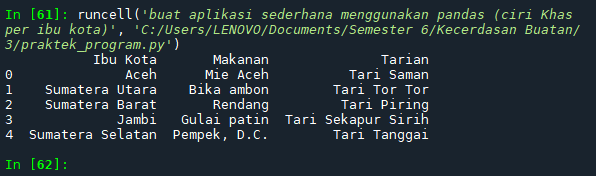
\includegraphics[width=10cm,height=4cm]{figures/Cp3-1.png}
    \caption{Aplikasi sederhana menggunakan pandas}
    \label{penanda}
\end{figure}
\textbf{Penjelasan Code Aplikasi Sederhana pandas perbaris :}
\begin{itemize}
    \item Langkah awal yaitu di line 1 merupakan langkah mengimport library pandas kemudian di inisialisasi menjadi pd
    \item Untuk bagian Variable data di definisikan data data untuk kolom nama, kolom npm dan kolom angkatan
    \item Pada bagian Variable frame itu akan berfungsi mengubah data pada variable data disejajarkan dengan baris dan kolom menggunakan pd dataframe
    \item Selanjutnya Peritah frame kemudian dijalankan untuk dapat menampilkan hasil dari dataframe
\end{itemize}

\subsection{Aplikasi Sederhana Menggunakan Matplotlib}
\begin{figure}[!htbp]
    \centering
    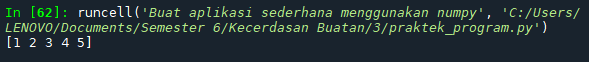
\includegraphics[width=10cm,height=2cm]{figures/Cp3-2.png}
    \caption{Aplikasi sederhana menggunakan matplotlib}
    \label{penanda}
\end{figure}
\textbf{Penjelasan Code Aplikasi Sederhana matplotlib perbaris :}
\begin{itemize}
    \item Baris Pertama Yaitu import library matplotlib kemudian di inisialisasi menjadi plt
    \item Variable prodi sebagai sumbu x untuk nama nama prodi
    \item Variable jumlah mhs sebagai sumbu y untuk jumlah atau banyaknya mahasiswa
    \item plt figure digunakan untuk mengatur size dan plt bar merupakan fungsi yang digunakan untuk memvisualisasikan bar
    \item plt title digunakan untuk memberikan judul dan plt ylabel untuk memberikan judul pada sumbu y
    \item plt yticks dan xticks digunakan untuk mengatur size tulisan pada sumbu y dan x
\end{itemize}

\subsection{Aplikasi Sederhana Menggunakan Numpy}
\begin{figure}[!htbp]
    \centering
    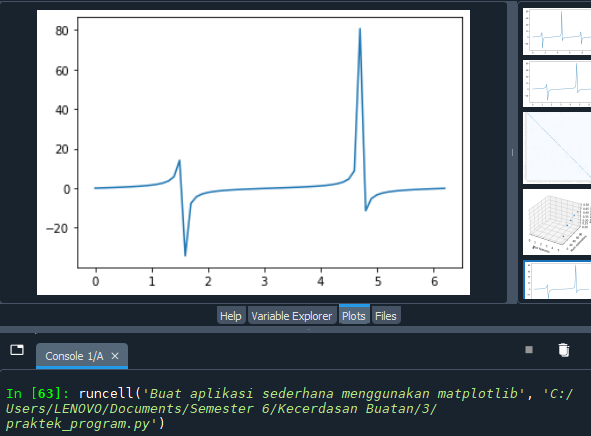
\includegraphics[width=6cm,height=6cm]{figures/Cp3-3.png}
    \caption{Aplikasi sederhana menggunakan numpy}
    \label{penanda}
\end{figure}
\textbf{Penjelasan Code Aplikasi Sederhana numpy perbaris :}
\begin{itemize}
    \item Baris Pertama Yaitu import library numpy kemudian di inisialisasi menjadi np
    \item Variable a digunakan sebagi fungsi array yang pertama
    \item Variable b digunakan sebagai fungsi array yang kedua
    \item Variable c digunakan sebagai fungsi array yang ketiga
    \item Perintah print digunakan untuk menampilkan hasil array
    \item Operasi pada array menggunakan perkalian pada a dan b dan penjumlahan pada b dan c
\end{itemize}


\section{Program Klasifikasi Random Forest}
Berikut merupakan output dari percobaan Random Forest yang telah dilakukan :
\begin{enumerate}

    \begin{figure}[!htbp]
        \centering
        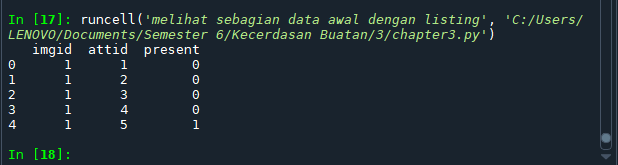
\includegraphics[width=12cm,height=6cm]{figures/Cp3-4.png}
        \caption{Membaca dataset file txt}
        \label{penanda}
    \end{figure}

    \item Kode berikut akan menampilkan output banyaknya jumlah baris dan kolom data frame imgatt
          \begin{figure}[!htbp]
              \centering
              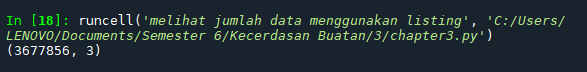
\includegraphics[width=4cm,height=1cm]{figures/Cp3-5.png}
              \caption{Mengetahui jumlah data}
              \label{penanda}
          \end{figure}

    \item imgatt2 menggunakan function pivot untuk merubah kolom menjadi baris dan baris menjadi kolom dari data frame sebelumnya.
          \begin{figure}[!htbp]
              \centering
              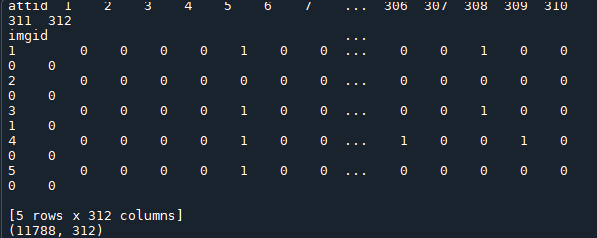
\includegraphics[width=12cm,height=2cm]{figures/Cp3-6.png}
              \caption{Pivot dataset}
              \label{penanda}
          \end{figure}

    \item Pada kode berikut digunakan dataset label kemudian akan diberi label pada burung dan menentukan burung tersebut ke dalam spesies apa. di dalam data yang sebelumnya ada 312 kolom dimana 312 data tersebut memiliki kelompoknya masing-masing. Dalam hal ini akan dimunculkan dua kolom pada variable explorer yaitu imgd dan label yang terdiri dari 11788 baris dan 1 kolom
          \begin{figure}[!htbp]
              \centering
              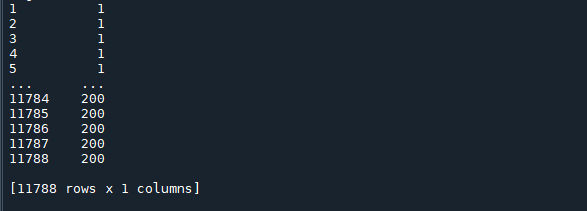
\includegraphics[width=12cm,height=2cm]{figures/Cp3-7.png}
              \caption{Membaca Dataset label}
              \label{penanda}
          \end{figure}

    \item Selanjutnya data imgatt2 akan join dengan imglabels atau menggabungkan field dari dua file yang terpisah, karena data baris sama banyak nya maka ditambahkan data kolom dari imgatt2 312 kolom dengan imglabels 1 kolom, maka hasilnya menjadi 313 kolom
          \begin{figure}[!htbp]
              \centering
              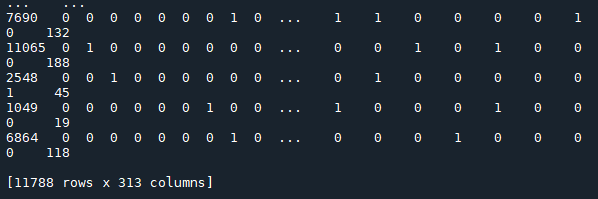
\includegraphics[width=7cm,height=2cm]{figures/Cp3-8.png}
              \caption{Menggabungkan field dari file yang terpisah}
              \label{penanda}
          \end{figure}

    \item Kemudian memisahkan dan memilih label atau memecah data kembali seperti sebelumnya dengan cara mengambil 312 dari belakang dan mengambil 312 dari depan.
          \begin{figure}[!htbp]
              \centering
              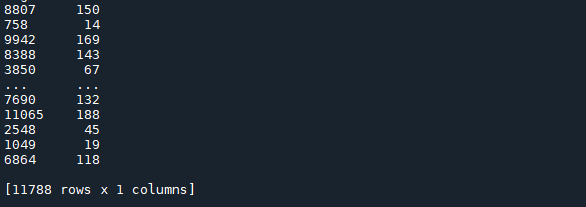
\includegraphics[width=7cm,height=2cm]{figures/Cp3-9.png}
              \caption{Memisahkan dan memilih label}
              \label{penanda}
          \end{figure}

    \item Membagi Data training dan data testing dengan mengambil row sebanyak 8000 dari akhir untuk training dan 8000 dari awal untuk data testing.
          \begin{figure}[!htbp]
              \centering
              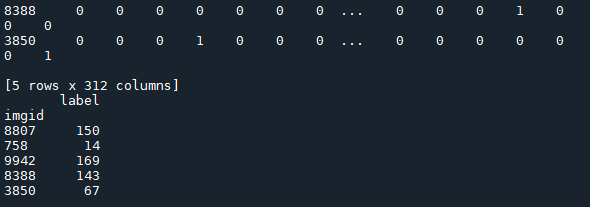
\includegraphics[width=7cm,height=3cm]{figures/Cp3-10}
              \caption{Pembagian data training dan tes}
              \label{penanda}
          \end{figure}

    \item Melakukan klasifikasi, di dalam kelas randomforestclassifier setting parameter variable yaitu 50 dalam satu independen tree maksimal akan mengakomodir 50 atribut. Kemudian lakukan instansiasi dengan melakukan klasifikasi pada data train att beserta data label nya.
          \begin{figure}[!htbp]
              \centering
              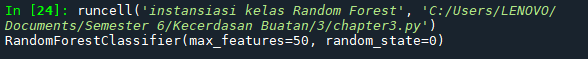
\includegraphics[width=14cm,height=3cm]{figures/Cp3-11}
              \caption{Instansiasi kelas Random Forest}
              \label{penanda}
          \end{figure}
\end{enumerate}

\section{Program Confusion Matrix}
Berikut merupakan output dari percobaan Confusion Matrix yang telah dilakukan :
\begin{enumerate}

    \item Selanjutnya plotting confusion matrix menggunakan matplotlib.
          \begin{figure}[!htbp]
              \centering
              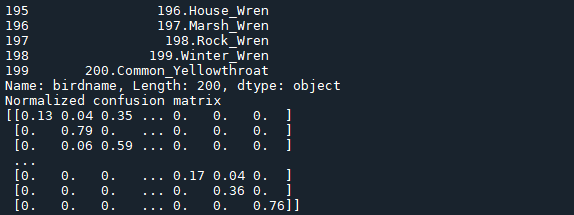
\includegraphics[width=11cm,height=11cm]{figures/Cp3-12.png}
              \caption{Plotting Confusion Matrix}
              \label{penanda}
          \end{figure}

    \item Membaca File Classes
          \begin{figure}[!htbp]
              \centering
              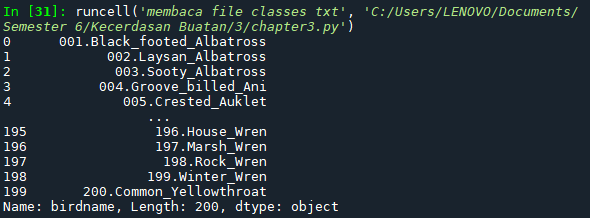
\includegraphics[width=11cm,height=5cm]{figures/Cp3-13.png}
              \caption{Membaca file classes}
              \label{penanda}
          \end{figure}

    \item Plot hasil perubahan label
          \begin{figure}[!htbp]
              \centering
              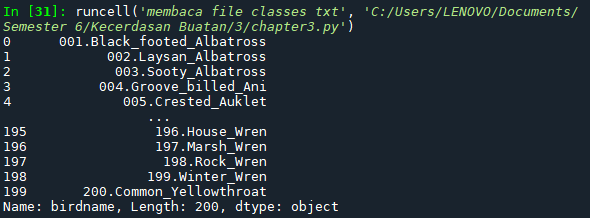
\includegraphics[width=10cm,height=4cm]{figures/Cp3-14.png}
              \caption{Plot hasil perubahan label}
              \label{penanda}
          \end{figure}
\end{enumerate}


\section{Program Klasifikasi SVM dan Decission Tree}
Berikut merupakan output dari percobaan Klasifikasi SVM dan Decission Tree yang telah dilakukan :
\begin{enumerate}
    \begin{figure}[!htbp]
        \centering
        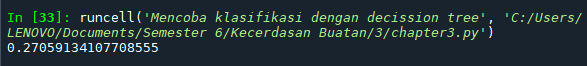
\includegraphics[width=8cm,height=2cm]{figures/Cp3-15.png}
        \caption{Klasifikasi Decission Tree}
        \label{penanda}
    \end{figure}

    \item Klasifikasi SVM dengan menggunakan dataset yang sama
          \begin{figure}[!htbp]
              \centering
              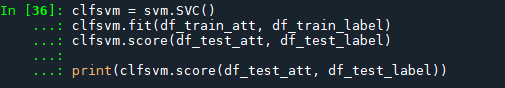
\includegraphics[width=8cm,height=2cm]{figures/Cp3-16.png}
              \caption{Klasifikasi SVM}
              \label{penanda}
          \end{figure}
\end{enumerate}

\section{Program Cross Validation}
Berikut merupakan output dari percobaan Program Cross Validation yang telah dilakukan :
\begin{enumerate}
    \item tugas minggu hari ini dan besok (maks 100). pada chapter ini
    \item presentasi decission tree (maks 100). Mempraktekkan kode python dan menjelaskan cara kerjanya.
    \item presentasi Random Forest (maks 100).Mempraktekkan kode python dan menjelaskan cara kerjanya.
    \item Hasil Cross Validation untuk Random forest
          \begin{figure}[!htbp]
              \centering
              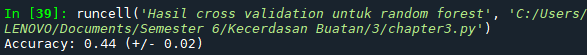
\includegraphics[width=14cm,height=2cm]{figures/Cp3-17.png}
              \caption{Hasil Cross Validation Random Forest}
              \label{penanda}
          \end{figure}
    \item Hasil Cross Validation untuk Decission Tree
          \begin{figure}[!htbp]
              \centering
              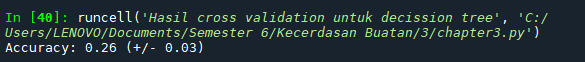
\includegraphics[width=14cm,height=1cm]{figures/Cp3-18.png}
              \caption{Hasil Cross Validation Decission Tree}
              \label{penanda}
          \end{figure}
    \item Hasil Cross Validation untuk SVM
          \begin{figure}
              \centering
              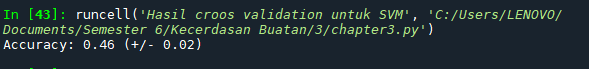
\includegraphics[width=14cm,height=1cm]{figures/Cp3-19.png}
              \caption{Hasil Cross Validation SVM}
              \label{penanda}
          \end{figure}
\end{enumerate}

\section{Program Pengamatan Komponen Informasi}
Berikut merupakan output dari percobaan Program Pengamatan Komponen Informasi yang telah dilakukan :
\begin{enumerate}
    \item Ouput berikut dapat mengetahui banyaknya tree yang dibuat, berapa atribut yang digunakan dan informasi lainnya.
          \begin{figure}
              \centering
              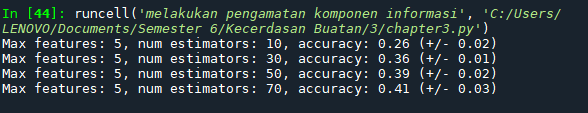
\includegraphics[width=11cm,height=5cm]{figures/Cp3-20.png}
              \caption{Hasil plotting komponen}
              \label{penanda}
          \end{figure}
    \item Output berikut merupakan hasil plotting komponen informasi agar dapat dibaca
          \begin{figure}
              \centering
              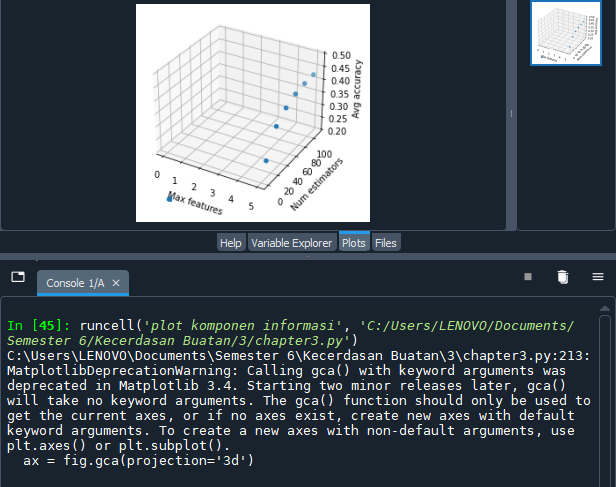
\includegraphics[width=8cm,height=9cm]{figures/Cp3-21.png}
              \caption{Hasil plotting komponen}
              \label{penanda}
          \end{figure}
\end{enumerate}